\setcounter{chapter}{2}
\chapter{Circuiti Elettrici}

\section{Condensatori}

In generale un condensatore \`e una coppia di conduttori che hanno carica Q e -Q rispettivamente. Un  esempio \`e dato da due piani conduttori in parallelo.

\subsection{Condensatore a piani paralleli}

\begin{wrapfigure}{r}{0.4\textwidth} % 'r' for right, 'l' for left
    \centering
    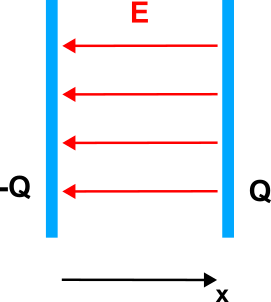
\includegraphics[width=0.3\textwidth]{images/parallelcapac} % Replace with your image
\end{wrapfigure}
Consideriamo due piani conduttori posti in parallelo come in figura, e assumiamo che la distanza $d$ tra i piani sia molto pi\`u piccola di $\sqrt{A}$ dove $A$ \`e l'area delle superfici planari. Imporre una condizione del genere ci permette di considerare gli effetti che si generano al bordo dei piatti e quindi possiamo assumere che il campo elettrico che generato nella regione tra i due piani coincide con quello che si avrebbe se le superfici avessero una estensione infinita. Il campo elettrico \`e dato da 
\begin{equation*}
	\bold{E} = -\frac{\sigma}{\varepsilon_0} \bold{\hat{x}}
\end{equation*}
dove $\sigma = Q/A$ e il campo ha direzione opposta a quella dell'asse $x$. Definiamo \textit{capacitanza} la grandezza 
\begin{equation}
	C = \frac{Q}{V}
\end{equation}
dove V rappresenta il $voltaggio$ o la \textit{differenza di potenziale}, tra i due piani paralleli. Dato che $\bold{E} = -\frac{d\phi}{dx}$, avremo che 
\begin{equation*}
	\phi(x) =-Ex+c \quad \Rightarrow \quad V = \phi(0) - \phi(d) = Ed = \frac{Qd}{A \varepsilon_0}
\end{equation*} 
e  quindi possiamo concludere che la capacitanza per due piatti paralleli di area A e posti ad una distanza $d$, sono
\begin{equation*}
	C = \frac{A \varepsilon_0}{d}
\end{equation*}
La capacitanza di un condensatore dipende dalla sua geometria e non dalla carica Q. I condensatori in generale vengo usati per immagazzinare energia elettrica. L'energia accumulabile da un condensatore \`e data dalla relazione 
\begin{equation*}
	U = \frac{1}{2} \varepsilon_0 \int_V dV \; \bold{E} \cdot \bold{E} = \frac{A \varepsilon_0}{2} \int_{0}^{d} dx \; \left ( \frac{\sigma}{\varepsilon_0}\right)^2 = \frac{Q^2}{2C}
\end{equation*}
L'unit\`a di misura per la capacitanza \`e data dal \textit{Farad} che \`e dato da 
\begin{equation*}
	[F] = \frac{[Coulomb]}{[Volt]}
\end{equation*}
Poich\`e la capacit\`a dei conduttori isolati ( e dei condensatori) sono proporzionali a $\varepsilon_0$ tramite una lunghezza (parametro di scala), torna utilie esprimere $\varepsilon_0$ in unit\`a di capacit\`a per unit\`a di lunghezza
\begin{equation*}
	\varepsilon_0 = 8,8 \times 10^{-12} \frac{F}{m}
\end{equation*}


Il condensatore planare che si \`e "ideale", ovvero \`e una trattazione semplificata che non tiene conto di alcune caratteristiche come gli effetti di bordo del campo elettrico che viene ipotizzato essere completamente contenuto all'interno del volume racchiuso tra le armature; 
\begin{wrapfigure}{l}{0.4\textwidth}
  \centering
  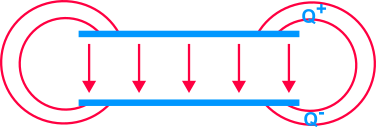
\includegraphics[width=0.38\textwidth]{images/edge_effect}
\end{wrapfigure}
questa semplificazione risulta essere pertinente con la realt\`a se la distanza tra i piatti $d \ll \sqrt{A}$ alla loro area o raggio se sono di natura circolare. 
\textit{In un disco conduttore isolato la distribuzione di carica $\sigma$ non \`e uniforme}, ma in una coppia di dischi ideali s\`i.
\newpage

\subsection{Conduttori con condensatore interno e esterno}

\begin{wrapfigure}{r}{0.4\textwidth}
  \centering
  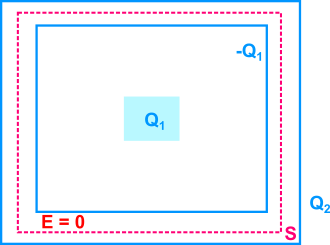
\includegraphics[width=0.38\textwidth]{images/cond_cons}
\end{wrapfigure}
Esempi di conduttori con all'interno condensatori sono i cavi coassiali. Per definizione la capacit\`a di un condensatore \`e data da 
\begin{equation*}
	C = \frac{Q_1}{\phi_1 - \phi_2}
\end{equation*}
dato che il campo nella cavit\`a dipende solo dalla carica $Q_1$. Per definizione il campo all'interno di un conduttore \`e nullo $\bold{E} = 0$ e di conseguenza anche il suo flusso $\phi_{S}(\bold{E}) = 0$, si ha dunque \textit{induzione completa}. Un eventuale carica $Q_2$ si distribuisce sulla superficie esterna. Possiamo vedere il sistema come due sotto sistemi uno costituito solo da $Q_1$ e uno costituito da $Q_2$ usando il principio di sovrapposizione di ottiene in il sistema di partenza. Il sistema che possiede solo $Q_2$ ha $\bold{E} =0$ all'interno della cavit\`a e dunque $Q_2$ \`e solo esterna. Il fatto che internamente il campo sia nullo nella configurazione in cui \`e presente solo $Q_2$, fa s\`i che il potenziale internamente sia costane 
\begin{equation*}
	\bold{E}_2 = - \nabla\phi_2 = 0 \Rightarrow \phi_2 = \text{cost}
\end{equation*}
di conseguenza nel sistema complessivo la differenza di potenziale dipende solo dal campo interno
\begin{equation*}
	\phi_{1} - \phi_2 = \int_{1}^{2} \bold{E}_{int} \cdot d\bold{s}
\end{equation*}
lungo un qualunque percorso tra i conduttori. Notare che $\phi_{2}$ \`e fissato dalle condizioni al contorno date dalla geometria della superficie esterna del conduttore.

\subsubsection{Esempio: Condensatore cilindrico}

Consideriamo un sistema formato da una distribuzione di carica lineare $\lambda = Q/L$ distribuita su un cilindro di raggio a, questo \`e racchiuso da un superficie cilindrica conduttrice di raggio b, dove $b>a$. Il campo elettrico interno \`e dato da 
\begin{equation*}
	E_{int} = \frac{\lambda}{2 \pi \varepsilon_0 } \frac{1}{r } \quad r \in [a,b]
\end{equation*}
e la differenza di potenziale \`e 
\begin{equation*}
	\varphi(a) - \varphi(b) = \int_{a}^{b} \bold{E} \cdot d\bold{s} = \frac{Q}{2 \pi \varepsilon_0 L } \log \left(\frac{b}{a}\right )
\end{equation*}
di conseguenza la capacit\`a \`e data da
\begin{equation*}
	C = \frac{Q}{\Delta \phi} = \frac{2 \pi \varepsilon_0 L}{\log \left(\frac{b}{a} \right)}
\end{equation*}

\subsection{Sistemi di conduttori (o condensatori a pi\`u strati)}

Consideriamo un sistema formato da N conduttori, per il quale ad infinito il potenziale vale $\phi = 0$. Prendiamo in analisi un singolo conduttore su cui \`e presente una carica $Q_i$, siccome un conduttore carico non interagisce con se stesso, la sua distribuzione di carica \`e legata al campo elettrico degli altri conduttori presenti nel sistema. Ovvero
\begin{equation*}
	\bold{E} = \sum_{i = 1}^{N-1}\bold{E}_i
\end{equation*} 
per il principio di sovrapposizione, la carica del condensatore \`e legata al campo dall Legge di Gauss dove 
\begin{equation*}
	\int_{S} \bold{E} \cdot d\bold{a} = \frac{Q_i}{\varepsilon_0} = \frac{1}{\varepsilon_0}\int_{V} \rho d\nu
\end{equation*}
utilizzando il teorema della divergenza si ha che 
\begin{equation*}
	\int_{S} \bold{E} \cdot d\bold{a}=\int_{V} (\nabla \cdot \bold{E}) \cdot d\nu
\end{equation*}
e dunque 
\begin{equation*}
	\nabla \cdot \bold{E} = \frac{\rho}{\varepsilon_0}
\end{equation*}
Dato che degli altri conduttori nel sistema conosciamo il potenziale possiamo esprimere la divergenza del campo elettrico, nell'equazione di Poisson 
\begin{equation*}
	\nabla^2\phi = - \frac{\rho}{\varepsilon_0}
\end{equation*}
dove ovviamente $\phi$ \`e il potenziale totale associato al campo $\bold{E}$. Per il teorema di unciti\`a la soluzione dell'equazione di Poisson \`e unica e questo ci garantisce che la carica sull'i-esimo conduttore \`e identificata in modo univoco. Poniamo il potenziale degli N-1 conduttori a $\phi_{i} = \phi (\infty) = 0$, in questo modo otteniamo una configurazione con un potenziale $\phi _1$ e un equazione di Laplace nel volume. Questa risulta essere risolubile con le adeguate condizioni al contorno.

Siccome $\phi_1$ determina in modo unico il campo elettrico, se raddoppiamo $\phi$ raddoppia anche $\bold{E}$ nel volume esterno al conduttore, di conseguenza raddoppiano anche le cariche $Q_1,Q_2,\ldots, Q_{k}$. Questo ci dice che la cariche di ciascun conduttore \`e proporzionale a $\phi_1$
\begin{equation*}
	Q_1 = C_{11}\phi_1 \quad Q_2 = C_{21}\phi_{1} \quad Q_3 = C_{31}\phi_{1} \quad \ldots \quad  Q_{N} = C_{N1}\phi_1
\end{equation*}
ripetendo lo stesso procedimento per ciascun conduttore, possiamo scrivere che le cariche dipendono da:
\begin{equation*}
	\left \{ \begin{array}{l}
		 Q_1 = C_{11} \phi_1 + C_{12}\phi_{2} + \ldots + C_{1N}\phi_{N} \\ \rule{0pt}{20pt}
		 Q_2 = C_{21} \phi_1 + C_{22} \phi_{2} + \ldots + C_{2N} \phi_N \\ \rule{0pt}{20pt}
		 \vdots \\ \rule{0pt}{20pt}
		 Q_{N} = C_{N1}\phi_{1} + C_{N2} \phi_2 + \ldots + C_{NN}\phi_{N}
	\end{array}\right.
\end{equation*}
I termine $C_{11},C_{22}, \ldots ,C_{NN}$ prendo il nome di \textbf{coefficienti di capacit\`a }, mentre i termini $C_{ij}$ con $i \neq j$ vengono chiamati \textbf{coefficienti di induzione}.

In forma matriciale 
\begin{equation*}
	\bm{Q} = \mathcal{C} \bm{\phi}
\end{equation*}
la matrice $\mathcal{C}$ \`e invertibile e simmetrica e quindi possiamo esprimere: 
\begin{equation*}
	\phi_{i} = \sum_{j}P_{ij}Q_{j}
\end{equation*}

\subsubsection{Collegamento a massa}

Mettere a massa consiste nel collegare (con un filo conduttore) un conduttore al riferimento per cui il potenziale $\phi = 0$. Il collegamento a terra fissa il potenziale a zero, ma non la carica (\`e  come se fosse presente una riserva di carica infinita all'infinito).
\newpage

\subsubsection{Esempio: collegamento a terra (Purcell 3.9)}
%Immagine QUI%
Consideriamo due sfere conduttrici cave A e B concentriche, dove il raggio $R_{A} < R_{B}$, e rispettivamente possiedono una carica $Q_{A} = Q$ e $Q_{B} = - Q$. Che cosa succede alla carica sulle due sfere  se la sfera B o la sfera A viene collegata a terra ?

\begin{proof}
\
\begin{itemize}
	\item 
	Consideriamo B a massa $\Rightarrow$ non cambia niente, il campo esterno \`e nullo, dunque 
	\begin{equation*}
		\phi_{B} = - \int_{\infty}^{R_{B}} \bold{E}_{ext} \cdot d\bold{r} = 0
	\end{equation*}
\item Se mettiamo A a massa $\phi_{A} = 0$ si ha in generale:
	\begin{equation*}
		\left \{ \begin{array}{l}
			\phi_{A} = P_{AA}Q_{A} + P_{AB} Q_{B} \\ \rule{0pt}{20pt}
			\phi_{B} = P_{BA}Q_{A} + P_{BB}Q_{B}
		\end{array}\right.
	\end{equation*}
Utilizzando il principio di sovrapposizione determiniamo i coefficienti del potenziale. Quindi studiamo un primo sistema in cui \`e presenta solo la carica   $Q_A \neq 0$, mentre $Q_{B} = 0$:
\begin{equation*}
	\left \{ \begin{array}{l}
		\phi_{A} = \frac{Q}{4 \pi \varepsilon_0} \frac{1}{R_{A}}\\ \rule{0pt}{20pt}
		\phi_{B} = \frac{Q_{A}}{4 \pi \varepsilon_0} \frac{1}{R_{B}}
	\end{array}\right.
\end{equation*}
dalle due equazioni segue che 
\begin{equation*}
	P_{AA} = \frac{1}{4 \pi \varepsilon_0 R_{A}} = \frac{1}{C_{AA}}  \quad \text{e} \quad P_{BA} = \frac{1}{4 \pi \varepsilon_0 R_{B}} 
\end{equation*}
Ripetiamo lo stesso ragionamento per $Q_{A} = 0$ e $Q_{B} \neq 0$:
\begin{equation*}
	\left \{ \begin{array}{l}
		\phi_{B} = \frac{Q_{B}}{4 \pi \varepsilon_0} \frac{1}{R_{B}} \\ \rule{0pt}{20pt}
		\phi_{A} = \phi_{B}
	\end{array}\right.
\end{equation*}
segue che 
\begin{equation*}
	P_{BB} = \frac{1}{4 \pi \varepsilon_0 R_{B}} = \frac{1}{C_{BB}} \quad \text{e} \quad P_{AB} = P_{BA}
\end{equation*}
sostituendo nelle equazioni del sistema
\begin{equation*}
	\phi_{A} = \frac{Q_{A}}{4 \pi \varepsilon_0} \frac{1}{R_{A}} + \frac{Q_{B}}{4 \pi \varepsilon_0}\frac{1}{R_{B}} = 0 \quad \Longrightarrow  \quad Q_{A} = - Q_{B}\frac{R_{A}}{R_{B}} = Q \frac{R_{A}}{R_{B}} < Q
\end{equation*}
Un po' di carica scappa ad infinito, per portare il potenziale a zero. Se non ne fluisse nemmeno un po' il potenziale sarebbe negativo, mentre se restasse tutta sarebbe positivo.
\end{itemize}
\end{proof}

\section{Conduttori Ohmnici}

\subsection{Legge di Ohm generalizzata}

Nei conduttori la carica si distribuisce in modo da annullare l'effetto del campo elettrostatico interno $\bold{E}_{int} = 0$. Quando si applica una differenza di potenziale lungo il conduttore, le cariche libere si mettono in moto creando una corrente, questo \`e dovuto al campo esterno $\bold{E}_{ext}$ del conduttore per mantenere il campo interno nullo.

Per la maggior parte dei materiali entro valori ampi di $\bold{E}$, si osserva una relazione empirica, detta \textbf{legge di Ohm}:
\begin{equation}
	\bold{J} = \sigma \bold{E}
\end{equation}
dove il termine $\sigma$ prende il nome di \textit{conducibilit\`a elettrica} di un mezzo; in generale \`e una grandezza scalare indipendente dalla direzione, ma ci sono alcuni materiali anisotropi che fanno da eccezione.

La relazione (3.2) \`e di natura vettoriale e include una convenzione di segno: \textit{	il verso di $\bold{J}$ \`e concorde con il verso del moto di trascinamento delle carica positive $\bold{J} = nq \bold{v}_{t}$}. Possiamo interpretare l'equazione (3.2) come quella di una forza viscosa che agisce su un punto materiale, dato che $\bold{E}$ moltiplicato per una carica \`e una forza:
\begin{equation*}
	q\bold{E} - q \frac{\bold{J}}{\sigma} = 0 \quad \iff \ddot{x} + \frac{nq^2}{m\sigma}\dot{x} = 0
\end{equation*}
Al posto di instaurarsi un moto uniformemente accelerato, si ha una un equilibrio delle forze dato dall'interazione Coulombiana tra le cariche instaurando un moto uniforme. L'attrito nel sistema possiamo immaginarlo come gli urti delle cariche con le cariche fisse nel volume, ed \`e uguale ovunque. Notare che c'\`e una differenza significativa  tra correnti elettriche:
\begin{equation*}
	I = JA
\end{equation*}
dove A \`e l'area della sezione del mezzo in cui scorre, e correnti idrauliche.

\begin{itemize}
	\item \textit{Corrente elettrica}: il flusso \`e indipendente dalla posizione nella sezione del mezzo, ovvero la velocit\`a \`e costante su tutta l'area A.
	\item \textit{Corrente idraulica}: il flusso segue un gradiente di velocit\`a che risulta essere nullo ai bordi e massimo al centro.
\end{itemize}
Possiamo domandarci se sia sensato assumere  che $\bold{J} $ sia costante lungo la sezione del conduttore, ma questa ipotesi \`e basata su un osservazione empirica in cui $\bold{E}$ risulta essere conservativo, ovvero a prescindere dal cammino scelto la differenza di potenziale che noi misuriamo in un mezzo \`e sempre la stessa, siccome empiricamente $\bold{J} = \sigma \bold{E}$ anche la densit\`a di corrente \`e conservativa e quindi uniforme sulla sezione del mezzo.
\newline

Numericamente possiamo vederlo considerando un filo di sezione A e lunghezza l, su cui misuriamo una differenza di potenziale $V$ ai due capi che indichiamo con a e b. Il lavoro compiuto per spostare una carica da un estremo all'altro \`e dato da
\begin{equation*}
	W = q V = \int_{a}^{b} \bold{E} \cdot d\bold{s} = El
\end{equation*}
Ipotizziamo  di calcolare lungo due percorsi $d\bold{l}_{1}$ e $d\bold{l}_{2}$ il lavoro necessario per spostare una carica dal punto a al punto b, e che il lavoro necessario \`e sempre lo stesso, ma il campo $E_1 \neq E_{2}$, avremmo che 
\begin{equation*}
	W_{1} =E_{1}l_{1} = E_{2}l_{2} = W_{2}
\end{equation*}
siccome $l_{1} = l_{2} \equiv l$ si ha che 
\begin{equation*}
	E_{1} = E_{2}
\end{equation*}
il che \`e assurdo. Dunque il campo deve essere uniforme e di conseguenza anche $\bold{J} = \sigma \bold{E}$ e quindi $\langle \bold{v} \rangle$ \`e costante i tutti  i punti della sezione.

Inoltre si hanno due ulteriori ipotesi:
\begin{itemize}
	\item Le distorsioni di campo per un conduttore finito sono trascurabili (buone se $L \gg A$, dove L \`e la lunghezza caratteristica e A l'area della sezione).
	\item Il conduttore non disperde carica dalle superfici laterali (buon isolamento).
\end{itemize}


\subsubsection{Conduttori non omogenei}

Per una corrente stazionaria $\nabla \cdot \bold{J} = 0$ e quindi $\nabla \cdot \bold{E} = 0$, il che vuol dire che in regioni di volume in cui la corrente \`e stazionaria non possono essere presenti distribuzioni di carica. Tale condizione risulta essere valida nel momento in cui $\sigma $ \`e una costante, nel caso in cui la conducibilit\`a non \`e omogenea $\sigma(x,y,z)$ si possono avere distribuzioni di carica locale statica.


Consideriamo un conduttore di sezione costante costituito da due materiali $\sigma_{1} \neq \sigma_{2}$ che al suo interno sia presente una densit\`a di corrente $\bold{J}$ stazionaria, allora deve valere che 
\begin{equation*}
	J_{1} = \frac{I}{A} = J_{2} \quad \Longrightarrow \quad \sigma_{1}E_{1} = \sigma_{2} E_{2} 
\end{equation*}
nei due mezzi si ha dunque che $E_{1} \neq E_{2}$ e quindi sulla superficie di separazione dei due materiali si ha una discontinuit\`a del campo elettrico. Questa discontinuit\`a fa s\`i  che crei della distribuzione di carica sulla superficie di separazione, data da 
\begin{equation*}
	\Delta E_{\bot} = \frac{\sigma}{\varepsilon_0} = \frac{Q}{A \varepsilon_0}  \quad \Longrightarrow \quad Q = A \varepsilon_0 \;\Delta E_{\bot} = \varepsilon_0 I \left(\frac{1}{\sigma_1} - \frac{1}{\sigma_2}\right)
\end{equation*}

\subsection{Modello corpuscolare e giustificazione delle legge di ohm generalizzata}

Esprimiamo la legge di Ohm generalizzata in modo esplicito rispetto alla velocit\`a media di deriva delle cariche nel conduttore, ottenendo l'equazione

\begin{equation*}
	Nq \langle \bold{v} \rangle = \sigma \bold{E}
\end{equation*}
abbiamo visto come a meno di un termine di carica questo dia origine a un comportamento viscoso con $\langle \bold{v} \rangle$ proporzionale alla forza di trascinamento sulle cariche.
\begin{equation*}
	\bold{F}_{T} = k \bold{v} = q \bold{E} = \bold{F}_{C}
\end{equation*}
Il moto di trascinamento \`e sovrapposto al moto di agitazione termica che avviene in modo molto pi\`u rapido. Per il moto di agitazione termica ipotizziamo che le cariche interagiscono nel seguente modo:
\begin{itemize}
	\item collisioni elastiche
	\item la direzione di $\bold{v}$ \`e casuale dopo ogni urto
\end{itemize}
Nel mezzo tra un urto e l'altro interviene la forza esercitata sulle cariche dal campo elettrico, contribuendo alla variazione della quantit\`a di moto.

Dopo ogni urto $\bold{p} = m \bold{v}_{c}$ con  direzione casuale, essendo gli urti elastici la variazione della quanti\`a di moto \`e conservata. Per quanto riguarda il contributo dato dalla forza Coulombiana, dal teorema dell'impulso abbiamo che 
\begin{equation*}
	\Delta \bold{p} = q\bold{E} \Delta t
\end{equation*}
Se osserviamo lo stato della carica ad un tempo $t_i$ dopo un urto, questa ha una quantit\`a di moto complessiva:
\begin{equation*}
	\bold{p_i} = m\bold{v}_{c,i} + q\bold{E}t_i
\end{equation*}
Se osserviamo il conduttore ad un tempo t prima dell'urto successivo, ciascun portatore avr\`a un momento $\bold{p}_{i}$ legato alla velocit\`a $\bold{v}_{c,i}$ ricevuta nell'urto e al tempo $t_i$. Calcoliamo il valore medio della velocit\`a per N portatori di carica:

\begin{equation*}
	m \langle \bold{v} \rangle = \frac{1}{N} \sum_{i}(m \bold{v}_{c,i} + q \bold{E} \;t_i) = m \langle \bold{v}_{c,i} \rangle  + q \bold{E} \;\tau_{M}
\end{equation*}
dove $\langle \bold{v}_{c,i} \rangle$ \`e la velocit\`a media dopo gli urti e $\tau_{M}$ \`e il tempo medio tra le collisioni (tempo di decorrelazione). Siccome la velocit\`a delle particelle dopo gli urti \`e casuale $\langle \bold{v}_{c,i} \rangle = 0$ e quindi la velocit\`a media (di deriva) dei portatori di carica \`e data da
\begin{equation*}
	\langle \bold{v} \rangle = \frac{\tau_{M} q}{m} \bold{E}
\end{equation*}
e quindi la densit\`a di corrente \`e data da 
\begin{equation*}
	\bold{J} = Nq \langle \bold{v} \rangle = \left(\frac{N \tau_{M} q^2}{m}\right)\bold{E} = \sigma \bold{E}
\end{equation*}
nel caso si abbia diversi portatori di carica si ha una sommatoria su $N_i$. 

La descrizione corpuscolare non \`e accurata a livello quantistico.
\subsection{Legge ohm per i circuiti elettrici}

La relazione generale tra $\bold{J}$ e $\bold{E}$ pu\`o essere ridotta nelle configurazioni di filo conduttore (o in geometrie definite) alla relazione empirica
\begin{equation}
	V = RI
\end{equation}
dove V \`e la differenza di tensione ai capi del conduttore e R \`e la resistenza elettrica  la cui unit\`a di misure \`e data dall' Ohm $[\Omega] = [V][A]^{-1}$. Per via empirica variando le configurazioni geometriche, si pu\`o rimuovere la dipendenza dalla geometria e introdurre una grandezza caratteristica del materiale, che esprime la reistenza elettrica del conduttore
\begin{equation*}
	R = \rho \; \frac{L}{A}
\end{equation*}
dove L \`e la lunghezza del mezzo e A l'area della sezione. Il termine $\rho$ prende il nome di \textbf{resistivit\`a} ed caratteristico del materiale.


La legge di Ohm vale per tutti i mezzi e per $\bold{E}$ non troppo intensi. il valore di $\rho$ permette di distinguere i materiali

\begin{table}[!ht]
\centering
\begin{tabular}{|l|l|l|}
\hline
\textbf{Categoria} & \textbf{Materiale} & \textbf{Resistivit\`a ($ \Omega \cdot m$)} \\
\hline
{Metalli} 
& Argento (Ag) & $1.62 \times 10^{-8}$ \\
& Rame (Cu) & $1.68 \times 10^{-8}$ \\
& Oro (Au) & $2.35 \times 10^{-8}$ \\
& Alluminio (Al) & $2.75 \times 10^{-8}$ \\
& Tungsteno (W) & $5.25 \times 10^{-8}$ \\
& Ferro (Fe) & $9.68 \times 10^{-8}$ \\
\hline
{Semiconduttori} 
& Silicio puro (Si) & $2.5 \times 10^{3}$ \\
& Germanio (Ge) & $\sim 5 \times 10^{1}$ \\
\hline
{Composti ionici} 
& Acqua di mare & $2.00 \times 10^{-1}$ \\
& Acqua potabile & $2.00 \times 10^{1} - 2.00 \times 10^{3}$ \\
\hline
{Isolanti} 
& Vetro & $10^{10} -10^{14}$ \\
& Quarzo fuso & $\sim 10^{16}$ \\
& Teflon & $10^{22}-10^{24}$ \\
\hline
\end{tabular}
\caption{Resistivit\`a elettrica di vari materiali a temperatura ambiente}
\end{table}

La resistivit\`a di un conduttore \`e legata alla sua conducibilit\`a mediante la relazione 

\begin{equation*}
	\rho = \frac{1}{\sigma}
\end{equation*}

la sua dimostrazione \`e semplice basta considerare un conduttore come un filo la cui superficie delle due estremit\`a formano dei piatti paralleli di area A, posti a distanza L , questo ci dice che il campo elettrico 
\begin{equation*}
	E = \frac{V}{L} \quad \text{e} \quad J = \frac{I}{A}
\end{equation*}
dalla legge di ohm generale abbiamo che 
\begin{equation*}
	\sigma \frac{V}{L} = \frac{I}{A} \quad \Longrightarrow \quad V = \left( \frac{L}{\sigma A}\right)I \quad \Rightarrow \quad \rho = \frac{1}{\sigma}
\end{equation*}

\section{Sistemi elettrici ed elementi circuitali}

\subsection{Circuiti resistivi}
La resistenza elettrica di un sistema pu\`o essere "ingegnerizzata" scegliendo materiali e geometria ( o combinazioni). Nella maggior parte dei casi non \`e necessario conoscere questi dettagli; la conoscenza di $R = V/I$ \`e sufficiente a caratterizzare il comportamento elettrico di un sistema. Un sistema completamente caratterizzato da R, prende il nome di \textit{apparecchio elettrico resistivo}; per queste tipologie di sistemi non ci interessa sapere come sono combinati gli elementi che lo costituiscono, ma \`e sufficiente sapere la tensione ai capi dei due terminali e la corrente che fluisce al suo interno. 

Il rapporto V/I caratterizza completamente l'apparecchio, nel caso in cui si abbiano correnti stazionarie (continue) e conduttori ohmnici. Per le correnti alternate (variabili nel tempo) \`e necessario qualche accorgimento.

\begin{wrapfigure}{r}{0.4\textwidth}
  \centering
  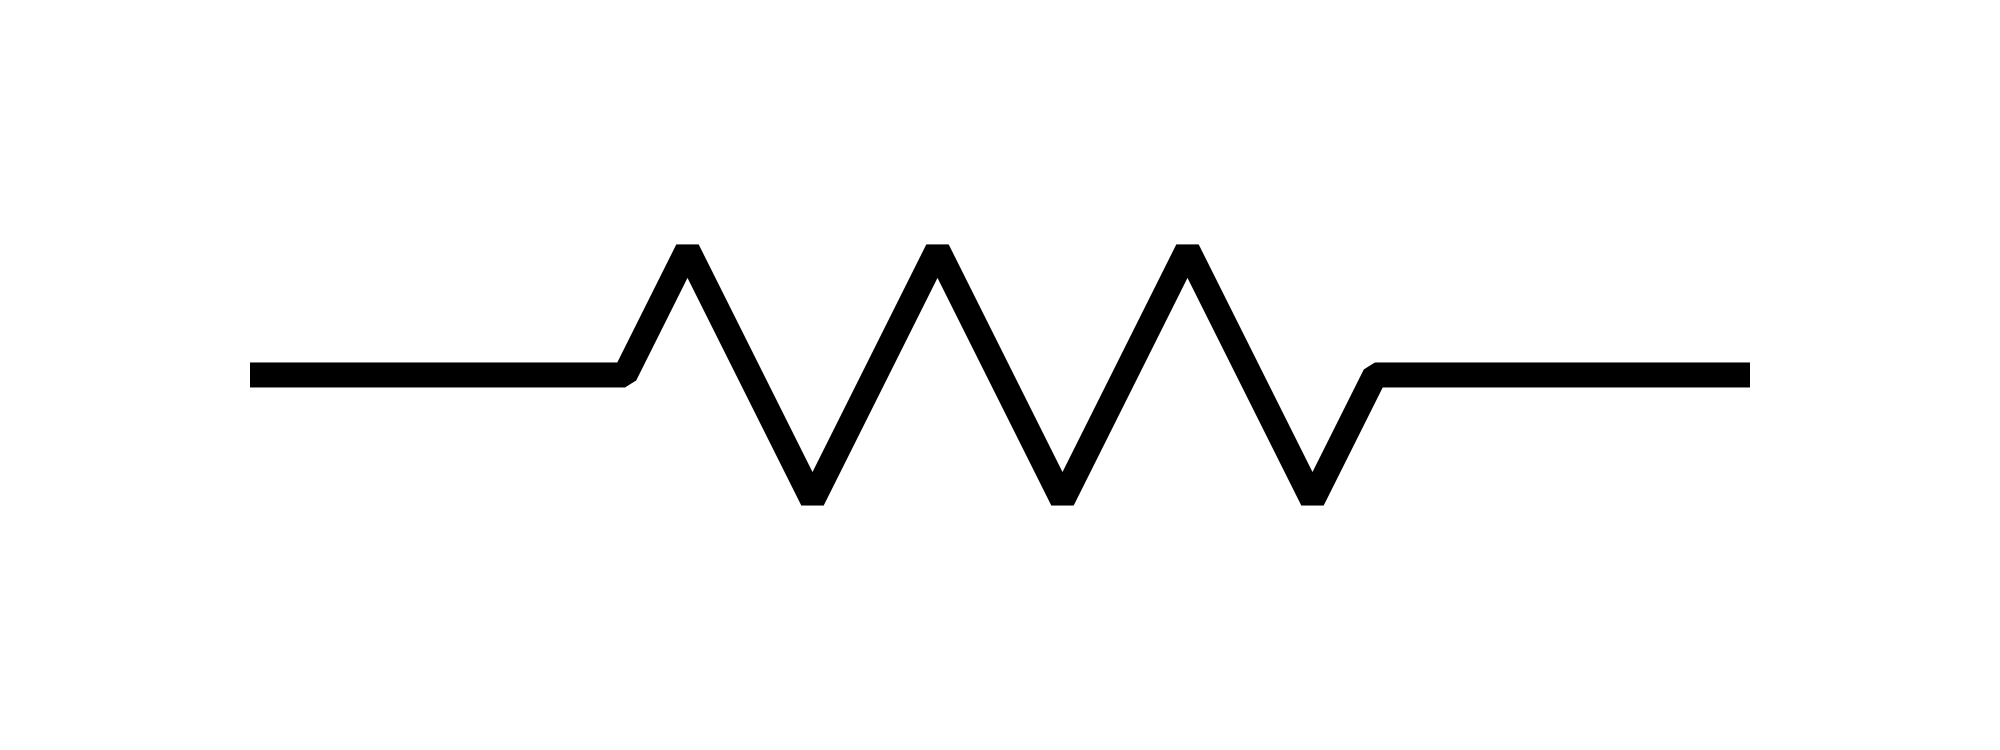
\includegraphics[width=0.38\textwidth]{images/resist}
  \caption{Raffigurazione dell'elemento circuitale della resistenza.}
\end{wrapfigure}

Un apparecchio elettrico resistivo prende anche il nome di circuito e pu\`o essere scomposto in elementi semplici. Definiamo \textbf{circuito resistivo}: una rete di resistenza connesse da fili di resistenza nulla. Ciascuna componente \`e caratterizzata dalla relazione $V = RI$.

\subsubsection{Resistenza in serie }
\begin{center}
	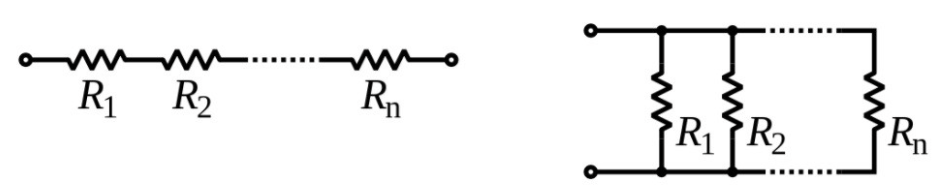
\includegraphics[width = \textwidth]{images/resist_serie}
\end{center}
All'interno di un circuito le resistenze possono assumere due configurazioni possibili, in \textbf{serie} e in \textbf{parallelo}.

Nel caso della configurazione in parallelo si ha che per una corrente I stazionaria e l'additivit\`a del potenziale
\begin{equation*}
	V  = \sum_{i=1}^N V_{N} = \sum_{i=1}^{N} R_{i}I =RI \quad \Rightarrow \quad R = \sum_{i=1}^{N} R_{i}
\end{equation*}
Se le resistenze si trovano in parallelo, la corrente I che scorre al loro interno anche se costante, si divide in ciascun nodo e dunque non \`e la medesima in ogni elemento circuitale, mentre la tensione V \`e la medesima per ognuno. Di conseguenza, dato:
\begin{equation*}
	I = \sum_{i=1}I_i = \sum_{i} \frac{1}{R_{i}}V = \frac{V}{R} \quad \Rightarrow \quad \frac{1}{R} = \sum_{i=1}^{N} \frac{1}{R_{i}}
\end{equation*}
\newpage
\subsubsection{Esempio: riduzione di un circuito}

\begin{wrapfigure}{l}{0.5\textwidth}

  \centering
  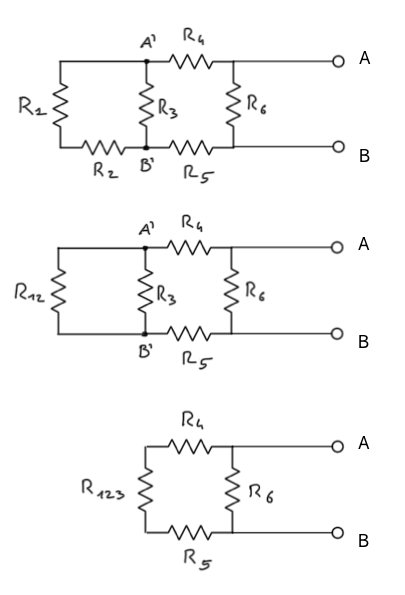
\includegraphics[width=0.49\textwidth]{images/redux1}
\end{wrapfigure}
La resistenza $R_{1}$ e $R_{2}$ sono in serie rispetto ai termini $A'$ e $B'$, di conseguenza possiamo calcolare una resistenza equivalente data da 
\begin{equation*}
	R_{12} = R_{1} + R_{2}
\end{equation*}
Nel nuovo circuito ridotto le resistenze $R_{12}$ e $R_{3}$ sono in parallelo, dunque possiamo calcolare una resistenza equivalente
\begin{equation*}
	R_{123} = \frac{R_{3}R_{12}}{R_{3}+R_{12}} = \frac{R_{3}(R_{1} + R_{2})}{R_{1} + R_{2} + R_{3}}
\end{equation*}
Infine l'ultimo circuito ha le resistenze in serie e quindi 
\begin{equation*}
	R = R_5 + R_{4} + R_{123}
\end{equation*}
e la serie di resistenze \`e in paralello a $R_6$:
\begin{equation*}
	R_{tot} = \frac{R_{6}(R_5 + R_4 + R_{123})}{R_6 + R_{5} + R_{4} + R_{123}}
\end{equation*}

\subsubsection{Esempio: catena infinita di resistenze (cavo con dispersione)}

\begin{center}
	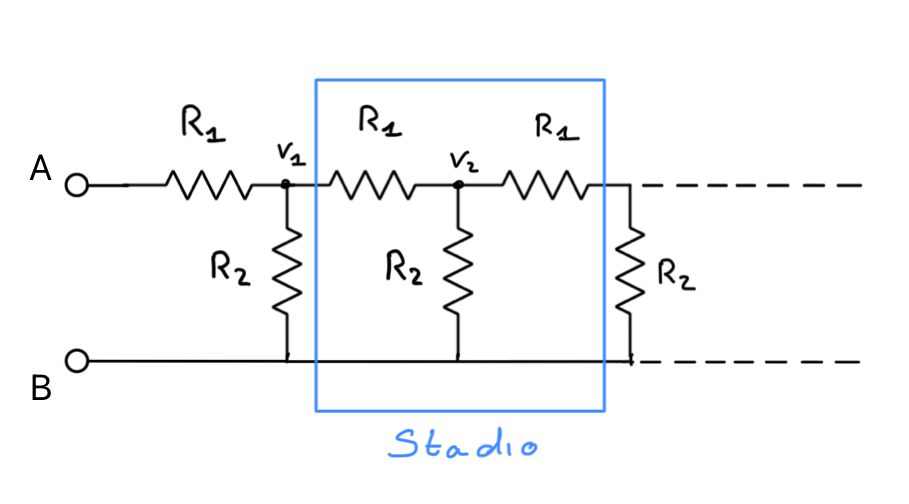
\includegraphics[width = 8 cm]{images/stadio}
\end{center}

\begin{itemize}
	\item Resistenza equivalente a quella del cavo di ingresso.
	\item Attenuazione del segnale dopo n-stadi.
\end{itemize}

Sia R la resistenza vista dai terminali A e B, se la catena \`e infinita, l'aggiunta di uno stadio non modifica il valore di R, dunque possiamo costruire una catena equivalente partendo dalle prime due resistenze.
\begin{center}
	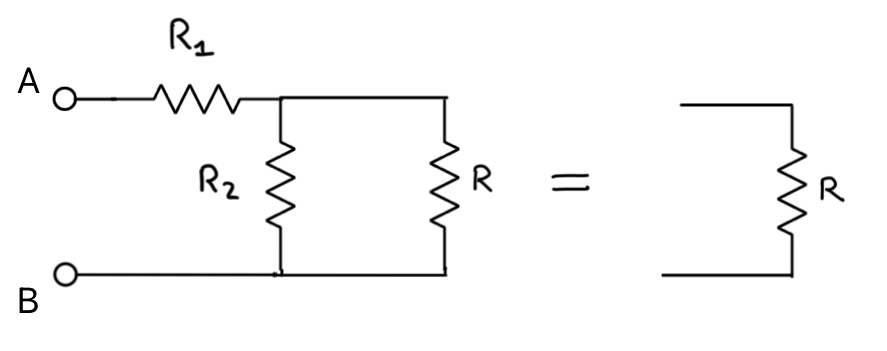
\includegraphics[width = 10cm]{images/redux3}
\end{center} 
 Dato che $R_1$ e $R_{2}$ sono in serie si ha una resistenza equivalente in parallelo ad R, e quindi la resistenza dello stadio \`e:
 \begin{equation*}
 	R_1 + \frac{R_2 R}{R_2 + R} + R \quad \Rightarrow \quad R = \frac{R_{1} + \sqrt{R_1^2 + 4R_{1}R_{2}}}{2}
 \end{equation*}
 Per ogni stadio vale quanto discusso per il calcolo di R e dunque la tensione sullo stadio \`e data da
 \begin{equation*}
 	V_{n} = \frac{R_{2}R}{R_{2} +R}I  \quad \text{e} \quad V_{n-1} = R_{1} + \frac{R_2R}{R_{2}+R} =R I
 \end{equation*}
di conseguenza
\begin{equation*}
	V_{n} = \frac{R_2R}{R_{2} + R}V_{n-1}
\end{equation*}
ripetendo in modo ricorsivo i passaggi si ha che 
\begin{equation*}
	V_{n} = \left(\frac{R_{2}R}{R_{2} + R}\right)^nV_{0}
\end{equation*}
dove $V_{0}$ \`e la tensione letta ai capi dei terminali.
 
 Nella pratica non \`e possibile costruire una catena infinita, ma possiamo chiudere le resistenze $R_{1}$ e $R_{2}$ con una resistenza R trovata nella discussione iniziale; in questo modo si ottiene un attenuatore con attenuazione variabile.
 
 \subsection{Leggi di Kirchhoff}
 
 Non tutte le reti o resistenze possono essere ridotte a combinazioni in serie o in parallelo. Se consideriamo il seguente circuito in figura, $R_{1}$ e $R_{2}$ non sono in parallelo perch\`e la tensione $V_{C} \neq V_{D}$. Analogamente $R_{5}$ e $R_{3}$ non sono in parallelo, non \`e nemmeno possibile individuare una serie.
 
 \begin{wrapfigure}{r}{0.4\textwidth}
  \centering
  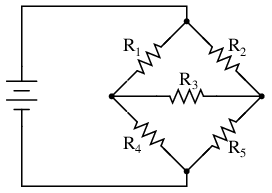
\includegraphics[width=0.38\textwidth]{images/kirch}
\end{wrapfigure}
 Per risolvere configurazioni come queste si ricorre alle relazione generali legate alle leggi fondamentali dell'elettrostatica e delle correnti stazionarie:
\begin{itemize}
	\item \textit{il campo elettrico \`e conservativo}: il valore del campo elettrico $\bold{E}$ lungo una linea chiusa (maglia) \`e nullo (il campo \`e conservativo).
	\item \textit{la carica \`e conservata} ossia vale l'equazione di continuit\`a 
	\begin{equation*}
		\nabla \cdot \bold{J} \; + \; \frac{\partial \rho}{\partial t} = 0
	\end{equation*}
	Nel caso stazionario sappiamo che $I = cost $ e quindi $\nabla \cdot \bold{J} = 0$ attraverso sezioni complete del circuito.
\end{itemize}
Queste relazioni si traducono nelle \textbf{leggi di Kirchhoff}:
\begin{enumerate}
	\item la somma della differenza di potenziale lungo una maglia qualunque \`e nulla 
	\begin{equation*}
		\sum_{i} V_i = 0
	\end{equation*}
	\item la somma algebrica delle correnti ai nodi del circuito \`e nulla 
	\begin{equation*}
		\sum_{i} I_{i} = 0
	\end{equation*}
\end{enumerate}
Nel sistema usato nell'esempio si hanno 4 nodi (i punti di congiunzione tra le componenti del circuito) e 3 maglie, usando le leggi di Kirchhoff si hanno 7 relazioni che legano le correnti.

\section{Forza elettromotrice nei circuiti}

Per sostenere la corrente in circuito resistivo (al cui interno come si \`e visto sono presenti forze dissipative)  occorre mantenere una differenza di potenziale $V_{AB}$
 nel tempo. Per farlo \`e necessario rimuovere la carica positiva dal polo B (negativo) e iniettarla in ingresso in A (polo positivo). La carica positiva deve muoversi contro il campo elettrico presente tra i due poli. 
 
 Il lavoro necessario per spostare le cariche positive deve essere erogato da una forza esterna di natura non elettrica; questo \`e dovuto al fatto che l'azione del campo elettrico sulle cariche positive le sposterebbe nella direzione opposta a quella necessaria. 
 
 \begin{wrapfigure}{l}{0.4\textwidth}
  \centering
  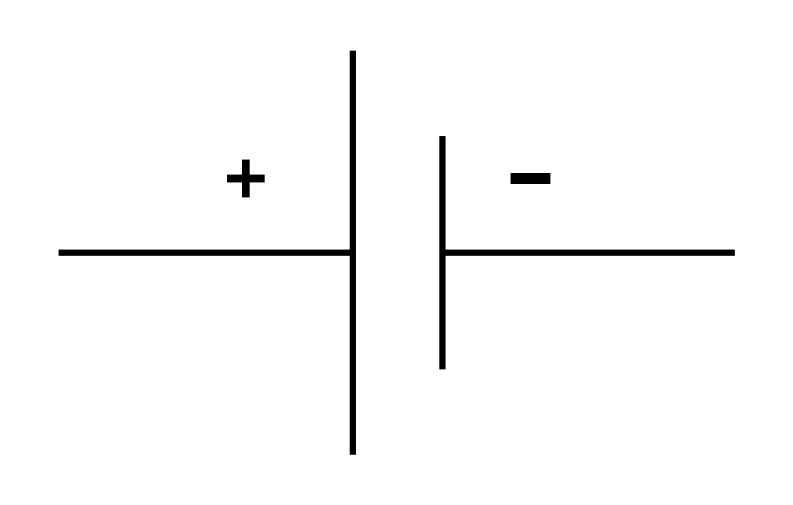
\includegraphics[width=0.3\textwidth]{images/fem}
  \caption{Raffigurazione dell'elemento circuitale della fem.}
\end{wrapfigure}
 Questa forza prende il nome di \textbf{forza elettromotrice (fem)} anche se in realt\`a non \`e una forza, ma il lavoro per unit\`a di carica compiuto per spostare le cariche. 
 In modo esplicito la fem \`e data da 
 \begin{equation}
 	\mathcal{E} = \oint_{C} \bold{f} \cdot d\bold{s} 
 \end{equation}
 dove $\bold{f}$ \`e la forza totale  per unit\`a di carica. In circuito chiuso le cariche sono soggette alla forza 
 \begin{equation*}
 	\bold{f} = \bold{f}_{s} + \bold{E}
 \end{equation*}
dove $\bold{f}_{s}$ \`e la forza esterna per unit\`a di carica dovuta alla fem. Riscrivendo (3.4):
\begin{equation*}
	\mathcal{E} = \oint_{C} \bold{f}_{s} \cdot d\bold{s} + \oint_{C} \bold{E} \cdot d \bold{s} = \oint_{A}^{B} \bold{f}_{s} \cdot d\bold{s}
\end{equation*}   
Possiamo misurare il lavoro della forza $\bold{f}_{s}$ da B ad A tramite il lavoro del campo elettrico
\begin{equation}
	\mathcal{E} = - \int_{B}^{A} \bold{E} \cdot d \bold{s} = V_{AB}  \quad \Rightarrow \quad V_{AB} - \mathcal{E} = 0
\end{equation}
il segno meno \`e dovuto al fatto che si compie lavoro contro il campo elettrico. Il risultato in (3.5) ci porta a ridefinire le leggi di Kirchhoff:
\begin{itemize}
	\item La somma dei potenziali della maglia non \`e pi\`u nulla, ma si deve includere $\mathcal{E}$
	\begin{equation*}
		\sum_{i} V_i = \mathcal{E}
	\end{equation*}
	\item si ha un segno negativo se  il verso della corrente va dal polo negativo a quello positivo
\end{itemize}

\subsubsection{Esempi di f.e.m}
 \begin{wrapfigure}{r}{0.4\textwidth}
  \centering
  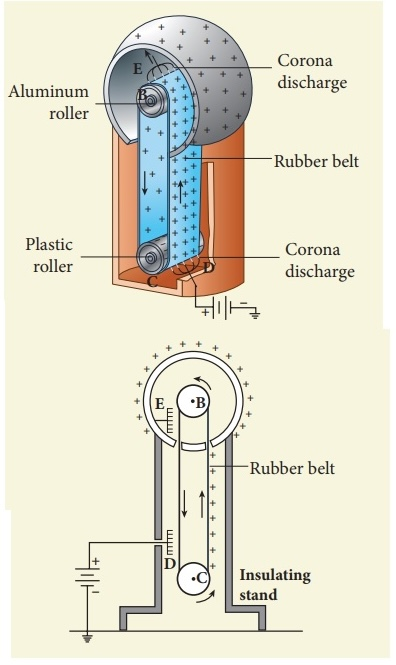
\includegraphics[width=0.39\textwidth]{images/van.jpg}
\end{wrapfigure}
1) \textbf{Macchina di Van de Graff}: si ha il trasporto della carica per via meccanica. Il macchinario \`e costituito da una cinghia isolante caricata per strofinamento, che viene messa in contatto con un pettine conduttore che raccoglie le cariche presenti su di essa. Il moto della cinghia \`e dovuto all'azione di un motore esterno. La carica \`e trasportata sul nastro in direzione opposta al campo elettrico.
\newline

\noindent 2) \textbf{Pile/cella voltaica}: Una reazione chimica con passaggio di elettroni da una molecola a un'altra sfruttando le differenze di energia di legame. Un esempio di batteria ancora usata \`e quello della batteria al piombo che \`e composta da diossido di piombo (elettrodi positivi), piombo metallico (elettrodi negativi) e una soluzione di acido solforico (elettrolita).

Nel funzionamento della pila gli ioni dell'idrogeno $H^+$ presenti nell'elettrolita si muovono verso il polo positivo, il campo elettrico ha verso in quel senso, con una discontinuit\`a di superficie. Questo accade perch\`e la reazione chimica \`e coveniente sotto il profilo energetico (rende pi\`u energia di quella spesa per muovere gli ioni $H^+$ contro il campo elettrico). In generale le pile possiedono una resistenza interna (contro il moto di $H^+$).

Quando si carica una batteria bisogna fornire l'energia spesa dalle reazioni chimiche (reazione inversa) e lavorare contro la resistenza interna per far migrare gli ioni verso l'altro elettrodo. Il lavoro contro la resistenza interna viene compiuto due volte e la spesa in energia \`e maggiore della resa.

\subsection{Potenza dissipata da elementi circuitali}

Abbiamo definito il lavoro compiuto per lo spsotamento di una carica in un campo elettrico come: 
\begin{equation*}
	W  = q\Delta V
\end{equation*}
e la potenza erogata 
\begin{equation*}
	P = \frac{dW}{dt} = \frac{dq}{dt} \Delta V = I \Delta V
\end{equation*}
sotto l'ipotesi che la differenza di potenziale $\Delta V$ sia mantenuta costante. Per un elemento circuitale come una resistenza, sappiamo che vale la legge di ogm 
\begin{equation*}
	\Delta V = RI
\end{equation*}
di conseguenza la potenza dissipata su di essa \`e data dalla relazione
\begin{equation}
	\frac{dW}{dt}= RI^2
\end{equation}
Tale risultato prende il nome di \textbf{effetto Joule} e rappresenta la potenza dissipata per via dell'attrito viscoso. L'energia cinetica acquisita dagli elettroni per effetto del lavoro del campo elettrico non si traduce in un trasporto netto (moto uniformemente accelerato), ma in un moto disordinato con direzione casuale.

Nella resistenza si ha che:
\begin{itemize}
	\item aumenta l'energia cinetica netta.
	\item la resistenza si scalda $\langle E\rangle  = \frac{3}{2}k_{B}T $
	\item L'energia viene dissipata sotto forma di calore. 
\end{itemize}
Per una forza elettromotrice la potenza erogata \`e data dal'equazione
\begin{equation*}
	\frac{dW}{dt}= I \mathcal{E}
\end{equation*}
\newpage

\subsection{Condensatori come elementi circuitali}
 \begin{wrapfigure}{l}{0.4\textwidth}
  \centering
  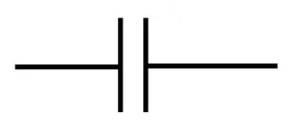
\includegraphics[width=0.39\textwidth]{images/cap}
  \caption{Capacitatore come elemento circuitale}
\end{wrapfigure}
Un condensatore pu\`o essere rappresentano come un elemento circuitale, le configurazioni che pu\`o assumere sono analoghe a quella che si sono viste per le resistenze, ovvero in serie e in parallelo. Abbiamo definito la capacit\`a di un condensatore come 
\begin{equation}
	C = \frac{Q}{V}
\end{equation}
\begin{center}
	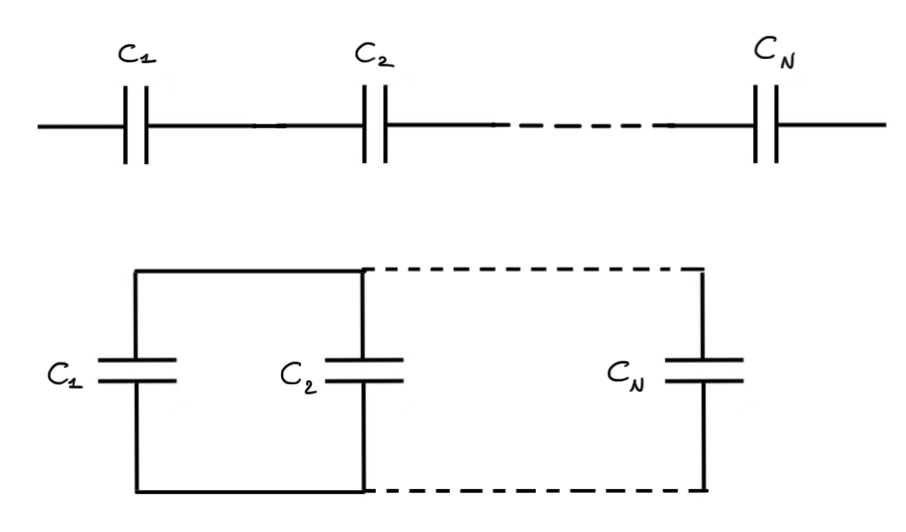
\includegraphics[width = 10cm]{images/cap_par_ser}
\end{center}
Nel caso di condensatori in \textbf{serie} la carica depositata sulle armature rimane invariata su ogni capacitatore $Q_1 = Q_2 =\ldots = Q_{N}$ e quello che cambia \`e la tensione, e quindi la tensione complessiva che misuriamo ai capi del circuito \`e data da:
\begin{equation*}
	V = V_{1} + V_{2} + \ldots + V_{N}
\end{equation*}
e usando la relazione (3.7) si ha che 
\begin{equation*}
	V = \frac{Q}{C_{eq}}= \frac{Q}{C_{1}} + \frac{Q}{C_{2}} + \ldots + \frac{Q}{C_{N}} = \left(\frac{1}{C_{1}} + \frac{1}{C_{2}} + \ldots + \frac{1}{C_{N}}\right)Q
\end{equation*}
e quindi 
\begin{equation}
	\frac{1}{C_{eq}} = \frac{1}{C_{1}} + \frac{1}{C_{2}} + \ldots + \frac{1}{C_{N}}
\end{equation}
Per in condensatori in \textbf{parallelo} questi sono collegati da fili  diversi che si raccordano al filo del circuito negli stessi punti. Come conseguenza di tale configurazione essi condividono lo stesso valore di differenza di potenziale $\Delta V$, mentre la carica totale \`e somma delle singole cariche 
\begin{equation*}
	Q = Q_{1} + Q_{2} + \ldots + Q_{N}
\end{equation*}  
Usando sempre la relazione (3.7) si ha:
\begin{equation*}
	Q = C_{eq} V = (C_1 + C_{2} + \ldots + C_{N})V \quad \Rightarrow \quad C_{eq} = C_{1} + C_{2} + \ldots + C_{N}
\end{equation*}
Il fatto che ogni condensatore abbia della carica differente possiamo vederlo dal fatto che in ciascuno di essi passa una corrente differente dagli altri dovendosi dividere su ciascun condensatore 
\begin{equation*}
	I = \frac{dQ}{dt} = \frac{d}{dt}(Q_{1} + Q_{2} + \ldots + Q_{N}) = I_{1} + I_{2} + \ldots + I_{N} 
\end{equation*}

\subsection{Carica e scarica di un condensatore }
\begin{wrapfigure}{l}{0.4\textwidth}
  \centering
  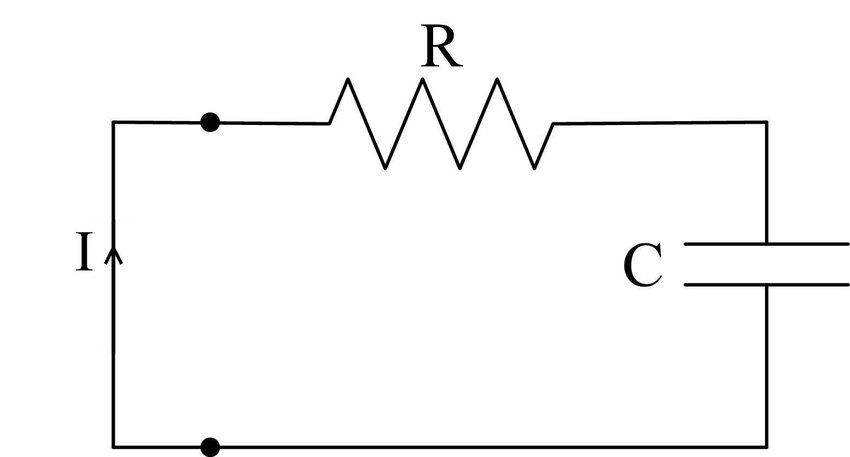
\includegraphics[width=0.39\textwidth]{images/RC_open}
\end{wrapfigure}
Consideriamo un circuito formato da una resistenza e un condensatore, e che il condensatore sia carico. Inizialmente il circuito \`e aperto e la tensione ai capi del condensatore al tempo $t = 0$ \`e $V(t) = V_0$. 

Nell'istante di tempo $t>t_0$ chiudiamo il circuito come in figura e lasciamo fluire la corrente al suo interno, dalle leggi di Kirchhoff sappiamo che per una maglia chiusa in cui non sono presenti forze elettromotrice la somma delle tensioni deve essere nulla:
\begin{align*}
	V_{C} + V_{R} = 0 \quad \iff \quad & V_{C}(t) + RI(t) = 0 \\ \rule{0pt}{20pt}
	& V_{C}(t) + RC\;\frac{dV}{dt} = 0 \quad \iff \quad \frac{dV}{dt} = - \frac{V}{RC}
\end{align*}
risolvendo l'equazione differenziale al primo ordine usando il metodo di separazione delle variabili e imponendo le condizioni iniziali si ha che 
\begin{equation*}
	V_{C}(t) = V_{0}e^{-t/RC} = V_0 e^{-t/\tau}
\end{equation*}
dove $\tau = RC$ ed \`e la costante di dimensione temporale e dipende dalle grandezze del circuito. Questo processo prende il nome di \textbf{scarica del condensatore}. Se vogliamo calcolare la variazione di energia immagazzinata nel condensatore abbiamo che:
\begin{equation*}
	\Delta U = U_{f} - U_{i} = \frac{1}{2}C V_{f}^2 - \frac{1}{2}CV_{i}^2 = - \frac{1}{2}CV_{0}^2
\end{equation*}
questa coincide con l'energia che viene dissipata sulla resistenza in calore, per via dell'effetto Joule:
\begin{equation*}
	W = \int_{0}^{+\infty} RI^2dt = \frac{V_{0}^2}{R} \int_{0}^{+\infty} e^{-2t/RC}dt = \frac{1}{2}C V_0^2
\end{equation*}
che coincide con l'energia ceduta dal condensatore.

\begin{wrapfigure}{r}{0.4\textwidth}
\vspace{-1cm}
  \centering
  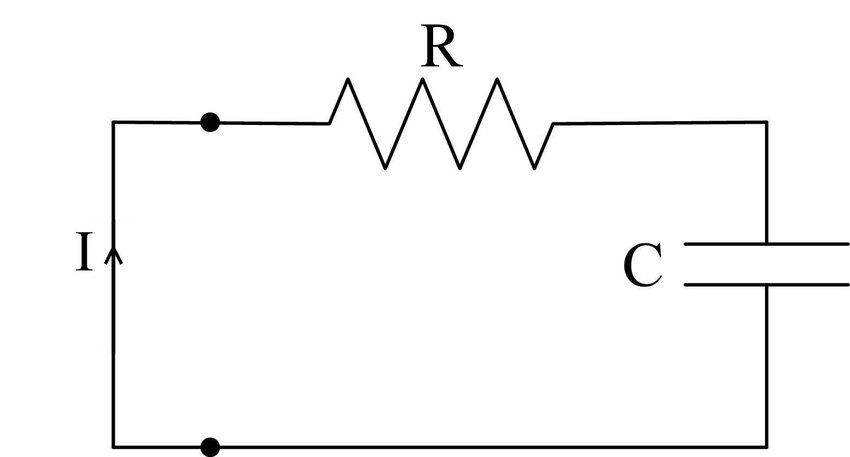
\includegraphics[width=0.39\textwidth]{images/RC_open}
\end{wrapfigure}

Viceversa se \textbf{vogliamo caricare un condensatore}, prendiamo il medesimo circuito solo che al suo interno \`e necessario avere un elemento in pi\`u dato dalla forza elettromotrice. Sempre utilizzando la legge di Kirchhoff e prendendo come condizioni al contorno $V(t=0) = 0$ abbiamo che: 
\begin{equation*}
	V_{C} + V_{R} = \mathcal{E} \quad \iff \quad V + RC\; \frac{dV}{dt} = \mathcal{E} 
\end{equation*}
la soluzione di questa equazione differenziale \`e data somma della soluzione dell'equazione omogenea e una soluzione particolare:
\begin{equation*}
	V_{C}(t) = \mathcal{E} (1-e^{-t/\tau})
\end{equation*}
dove $\tau = RC$. Da un punto di vista energetico la differenza di energia \`e data da 
\begin{equation*}
	\Delta U_{cond} = \frac{1}{2}C \mathcal{E}^2
\end{equation*}
e 
\begin{equation*}
	\Delta E_{fem} = \int_{0}^{+\infty} \mathcal{E}I dt  =\frac{\mathcal{E}^2}{R} \int_{0}^{+\infty} e ^{-t/RC} dt = C \mathcal{E}^2
\end{equation*}
che coincide con l'energia erogata dalla fem. Complessivamente l'energia dissipata sulla resistenza \`e data da:
\begin{equation*}
	\Delta E_{R} = \Delta E_{fem} - \Delta U_{cond} = \frac{1}{2}C \mathcal{E}_{2}
\end{equation*}
met\`a dell'energia \`e spesa sulla resistenza indipendentemente dal valore di R.

\subsubsection{Esempio: blocco di rame}

\begin{wrapfigure}{r}{0.4\textwidth}
\vspace{-1cm}
  \centering
  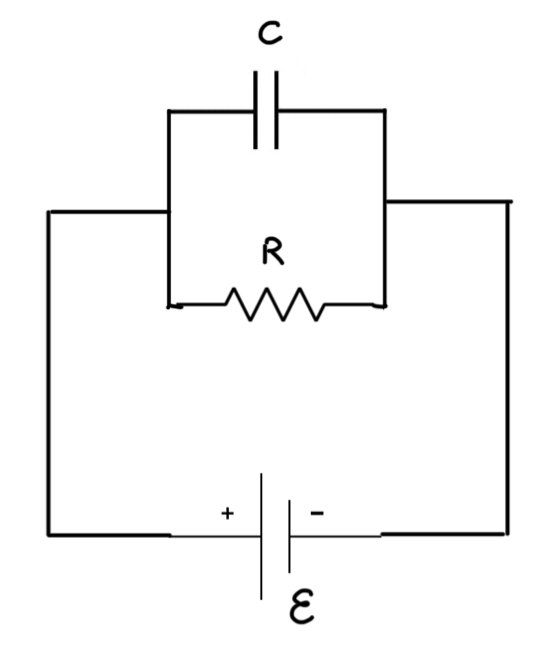
\includegraphics[width=0.39\textwidth]{images/rame}
\end{wrapfigure}
Consideriamo un blocco di rame che ha una resistivit\`a pari a $\rho  = 2 \times 10^8 \; \Omega \cdot m$, e lo colleghiamo a una forza elettromotrice. La configurazione sperimentale ottenuta \`e equivalente al circuito in figura.

Nel conduttore \`e presente una certa capacit\`a e una certa resistenza. Se inizialmente il sistema \`e aperto questo \`e neutro, ma nel momento in cui si chiude all'interno del conduttore si instaura un campo elettrico e un regime stazionario di corrente con della carica superficiale sulle estremit\`a.  Il tempo di risposta del sistema \`e dato da 
\begin{equation*}
	\tau = RC = \rho \frac{L}{A}\varepsilon_0\frac{A}{L} = \rho \varepsilon_0
\end{equation*}  
e si ha una costante di tempo che dipende completamente dalla resistivit\`a del materiale.



